% =============================================================================
% DSPRO2 Final Presentation: Pokemon Nuzlocke RL Agent
% Compile: pdflatex presentation.tex (2 passes for stable refs)
% =============================================================================
\documentclass[aspectratio=169, 11pt]{beamer}

% --- Theme & Colors ----------------------------------------------------------
\usetheme{Madrid}
\usecolortheme{default}

\definecolor{primaryBlue}{RGB}{10, 80, 160}
\definecolor{darkBlue}{RGB}{5, 50, 100}
\definecolor{accentOrange}{RGB}{230, 130, 30}
\definecolor{lightGray}{RGB}{240, 240, 245}
\definecolor{successGreen}{RGB}{40, 160, 60}
\definecolor{warnRed}{RGB}{200, 50, 50}

\setbeamercolor{palette primary}{bg=primaryBlue, fg=white}
\setbeamercolor{palette secondary}{bg=darkBlue, fg=white}
\setbeamercolor{palette tertiary}{bg=darkBlue, fg=white}
\setbeamercolor{structure}{fg=primaryBlue}
\setbeamercolor{title}{fg=white, bg=primaryBlue}
\setbeamercolor{frametitle}{fg=white, bg=primaryBlue}
\setbeamercolor{block title}{bg=primaryBlue, fg=white}
\setbeamercolor{block body}{bg=lightGray}
\setbeamercolor{block title alerted}{bg=warnRed, fg=white}
\setbeamercolor{block title example}{bg=successGreen, fg=white}
\setbeamercolor{item}{fg=primaryBlue}
\setbeamercolor{subitem}{fg=primaryBlue!70}

\setbeamertemplate{navigation symbols}{}
\setbeamertemplate{footline}{%
  \leavevmode%
  \hbox{%
    \begin{beamercolorbox}[wd=.333\paperwidth,ht=2.5ex,dp=1ex,center]{palette primary}%
      \usebeamerfont{author in head/foot}\insertshortauthor
    \end{beamercolorbox}%
    \begin{beamercolorbox}[wd=.334\paperwidth,ht=2.5ex,dp=1ex,center]{palette secondary}%
      \usebeamerfont{title in head/foot}\insertshorttitle
    \end{beamercolorbox}%
    \begin{beamercolorbox}[wd=.333\paperwidth,ht=2.5ex,dp=1ex,right]{palette tertiary}%
      \insertframenumber{} / \inserttotalframenumber\hspace*{2ex}
    \end{beamercolorbox}%
  }%
}

% --- Packages ----------------------------------------------------------------
\usepackage[T1]{fontenc}
\usepackage{lmodern}
\usepackage{booktabs}
\usepackage{tabularx}
\usepackage{tikz}
\usetikzlibrary{arrows.meta, positioning, shapes.geometric, fit, calc, backgrounds}
\usepackage{graphicx}
\usepackage{hyperref}
\usepackage{xcolor}
\usepackage{amsmath}
% --- Metadata ----------------------------------------------------------------
\title[Pok\'{e}mon Nuzlocke RL]{Training a Reinforcement Learning Agent\\for Pok\'{e}mon Nuzlocke Battles}
\subtitle{DSPRO2 Final Presentation}
\author[Muri, Hueber]{%
  Tristan Muri \and Marvin Hueber \\[0.3em]
  {\small Viacheslav Godovskii \quad Alex Liubov}}
\institute[HSLU]{Hochschule Luzern -- DSPRO2 FS26}
\date{May 2026}

% =============================================================================
\begin{document}

% --- Title Slide -------------------------------------------------------------
\begin{frame}[plain]
  \titlepage
\end{frame}

% --- Agenda ------------------------------------------------------------------
\begin{frame}{Agenda}
  \begin{enumerate}\setlength{\itemsep}{0.6em}
    \item \textbf{The Challenge} -- Nuzlocke rules, Pok\'{e}mon battles, milestones
    \item \textbf{Technical Setup} -- Architecture, tech stack, training flow
    \item \textbf{Model \& Training} -- Observation space, architecture, reward design
    \item \textbf{Development Journey} -- Critical bugs and breakthroughs
    \item \textbf{Results} -- Milestone~1 \& 2 outcomes
    \item \textbf{Live Demo}
    \item \textbf{Conclusions \& Next Steps}
  \end{enumerate}
\end{frame}

% =============================================================================
% SECTION 1: THE CHALLENGE
% =============================================================================
\section{The Challenge}

% --- Slide: Nuzlocke --------------------------------------------------------
\begin{frame}{What is a Pok\'{e}mon Nuzlocke?}
  A \textbf{self-imposed difficulty rule set} that transforms casual Pok\'{e}mon
  battles into a problem requiring long-horizon planning, risk assessment, and
  resource management:

  \vspace{0.5em}
  \begin{block}{Nuzlocke Rules}
    \begin{itemize}
      \item \textbf{First-catch:} Only the first Pok\'{e}mon encountered per
            location may be captured.
      \item \textbf{Permadeath:} Fainted Pok\'{e}mon are permanently lost.
      \item \textbf{Run failure:} Losing a battle ends the entire run.
    \end{itemize}
  \end{block}

  \vspace{0.5em}
  \textbf{Why this is interesting for RL:}
  \begin{itemize}
    \item Irreversible consequences create a \emph{sparse, high-stakes} reward
          landscape.
    \item Limited resources require strategic allocation across a sequence of
          battles.
    \item Partial observability (unknown opponent teams, hidden abilities).
  \end{itemize}
\end{frame}

% --- Slide: Pokemon Battles -------------------------------------------------
\begin{frame}{Pok\'{e}mon Battles in 30 Seconds}
  \begin{columns}[T]
    \begin{column}{0.55\textwidth}
      \textbf{Turn-based 6v6 singles:}
      \begin{itemize}\setlength{\itemsep}{0.4em}
        \item Each player brings up to 6 Pok\'{e}mon; 1 active at a time.
        \item Each turn: choose \emph{attack} or \emph{switch} (simultaneous,
              hidden).
        \item Execution order: move priority $>$ speed stat.
        \item Objective: faint all opponent Pok\'{e}mon.
      \end{itemize}

      \vspace{0.5em}
      \textbf{Type matchups stack multiplicatively:}

      \vspace{0.3em}
      \centering
      \small
      \begin{tabular}{ll}
        \toprule
        Modifier & Multiplier \\
        \midrule
        STAB (same-type bonus) & $\times 1.5$ \\
        Super effective        & $\times 2.0$ \\
        Resisted               & $\times 0.5$ \\
        Immune                 & $\times 0.0$ \\
        \bottomrule
      \end{tabular}
    \end{column}

    \begin{column}{0.42\textwidth}
      \begin{alertblock}{Why it's hard for RL}
        \begin{itemize}\setlength{\itemsep}{0.3em}
          \item Large state space (species, types, moves, items, abilities, boosts, weather, \ldots)
          \item Stochastic damage rolls
          \item Simultaneous hidden actions
          \item Partial observability of opponent team
          \item Long episodes ($\sim$25 turns)
        \end{itemize}
      \end{alertblock}
    \end{column}
  \end{columns}
\end{frame}

% --- Slide: Milestones ------------------------------------------------------
\begin{frame}{Milestone Roadmap}
  \begin{center}
    \small
    \begin{tabularx}{\textwidth}{c l X l}
      \toprule
      \textbf{\#} & \textbf{Milestone} & \textbf{Goal} & \textbf{Status} \\
      \midrule
      1 & Proof of Concept &
        Fixed team vs.\ random opponents. Tests whether the model can
        learn to use a known team. &
        \textcolor{successGreen}{\textbf{Solved}} \\
      2 & Random Battles &
        Randomly generated teams on both sides. Tests generalisation
        under high entropy. &
        \textcolor{accentOrange}{\textbf{In progress}} \\
      3 & Team Building &
        Learn to compose optimal teams given opponent information. &
        \textcolor{gray}{Future} \\
      4 & Gauntlet Master &
        Full Nuzlocke gauntlet completion (706 trainers). &
        \textcolor{gray}{Future} \\
      \bottomrule
    \end{tabularx}
  \end{center}

  \vspace{0.8em}
  \begin{alertblock}{Important}
    The project will \textbf{not} be completed within the scope of this module.
    Milestone~1 is essentially solved; Milestone~2 remains an open challenge.
    The project will continue beyond the course.
  \end{alertblock}
\end{frame}

% =============================================================================
% SECTION 2: TECHNICAL SETUP
% =============================================================================
\section{Technical Setup}

% --- Slide: Architecture Diagram --------------------------------------------
\begin{frame}{System Architecture}
  \centering
  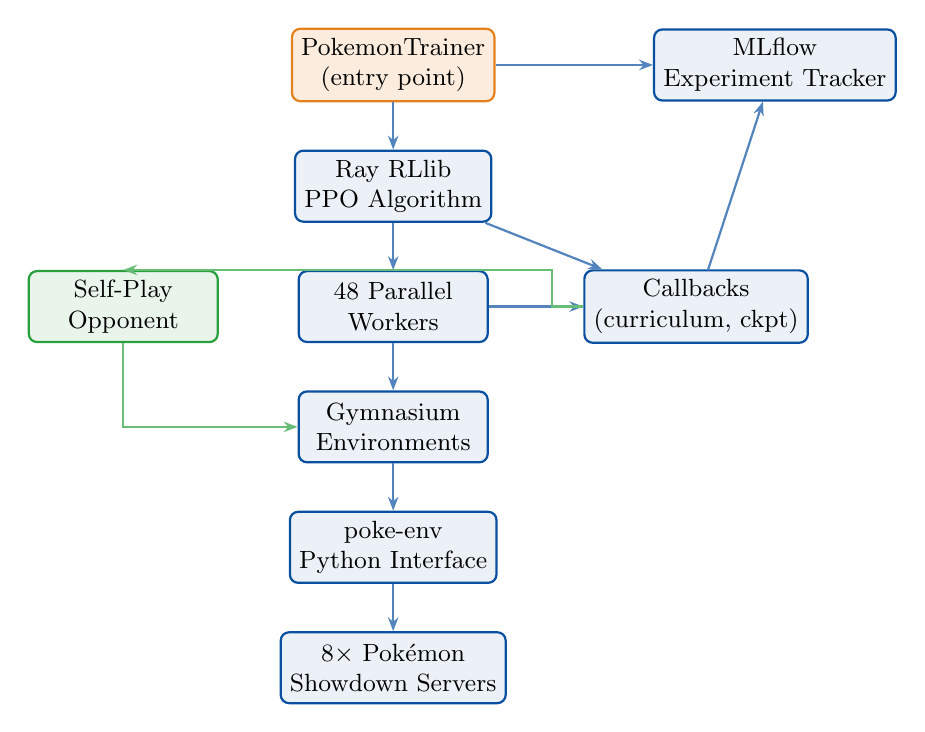
\begin{tikzpicture}[
    node distance=0.6cm and 1.2cm,
    box/.style={
      rectangle, draw=primaryBlue, fill=primaryBlue!8,
      rounded corners=3pt, minimum height=0.9cm, minimum width=2.4cm,
      font=\small, align=center, line width=0.8pt
    },
    arrow/.style={-{Stealth[length=5pt]}, thick, primaryBlue!70},
    label/.style={font=\scriptsize\itshape, text=gray}
  ]
    % Top level
    \node[box, fill=accentOrange!15, draw=accentOrange]
      (trainer) {PokemonTrainer\\(entry point)};

    % Second level
    \node[box, below=of trainer] (rllib) {Ray RLlib\\PPO Algorithm};
    \node[box, right=2cm of trainer] (mlflow) {MLflow\\Experiment Tracker};

    % Third level
    \node[box, below=of rllib] (workers) {48 Parallel\\Workers};
    \node[box, right=of workers] (callbacks) {Callbacks\\(curriculum, ckpt)};

    % Fourth level
    \node[box, below=of workers] (envs) {Gymnasium\\Environments};
    \node[box, below=of envs] (pokeenv) {poke-env\\Python Interface};
    \node[box, below=of pokeenv] (showdown) {8$\times$ Pok\'{e}mon\\Showdown Servers};

    % Arrows
    \draw[arrow] (trainer) -- (rllib);
    \draw[arrow] (trainer) -- (mlflow);
    \draw[arrow] (rllib) -- (workers);
    \draw[arrow] (rllib) -- (callbacks);
    \draw[arrow] (workers) -- (envs);
    \draw[arrow] (envs) -- (pokeenv);
    \draw[arrow] (pokeenv) -- (showdown);
    \draw[arrow] (callbacks) -- (mlflow);
    \draw[arrow] (workers.east) -- ++(0.4,0) |- (callbacks.west);

    % Self-play loop
    \node[box, left=1cm of workers, fill=successGreen!10, draw=successGreen]
      (selfplay) {Self-Play\\Opponent};
    \draw[arrow, successGreen!70] (callbacks.west) -- ++(-0.4,0) |- (selfplay.north);
    \draw[arrow, successGreen!70] (selfplay.south) |- (envs.west);
  \end{tikzpicture}
\end{frame}

% --- Slide: Tech Stack ------------------------------------------------------
\begin{frame}{Tech Stack \& Versions}
  \begin{center}
    \small
    \begin{tabularx}{0.92\textwidth}{l l X}
      \toprule
      \textbf{Component} & \textbf{Version} & \textbf{Role} \\
      \midrule
      Python        & 3.13          & Runtime \\
      PyTorch       & $\geq$2.10    & Neural network training \\
      Ray / RLlib   & $\geq$2.54    & Distributed RL orchestration \\
      poke-env      & $\geq$0.12    & Gymnasium interface to Showdown \\
      Pok\'{e}mon Showdown & self-hosted & Battle simulator (Node.js) \\
      MLflow        & $\geq$3.10    & Experiment tracking \& metrics \\
      Optuna        & $\geq$4.8     & Hyperparameter optimization (TPE) \\
      Gymnasium     & $<$1.2.3      & Environment API \\
      \midrule
      \multicolumn{3}{l}{\textbf{Hardware:} NVIDIA RTX 5090, 48 parallel
        environments, 8 Showdown instances (ports 8000--8007)} \\
      \bottomrule
    \end{tabularx}
  \end{center}

  \vspace{0.4em}
  \begin{itemize}
    \item Package management: \texttt{uv} with locked dependencies (\texttt{uv.lock})
    \item All code open-source; all dependencies permissively licensed
  \end{itemize}
\end{frame}

% --- Slide: Training Run Flow -----------------------------------------------
\begin{frame}{Training Run Flow}
  \centering
  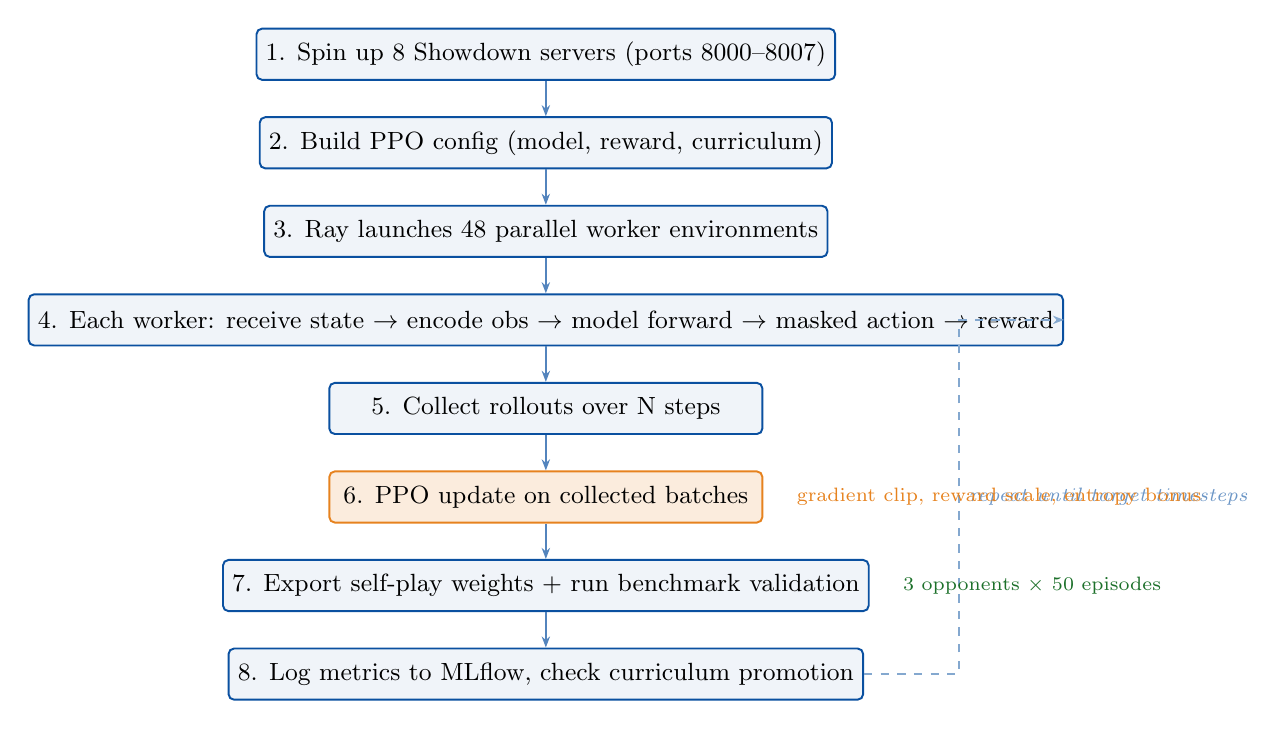
\begin{tikzpicture}[
    node distance=0.45cm,
    flowstep/.style={
      rectangle, draw=primaryBlue, fill=primaryBlue!6,
      rounded corners=2pt, minimum height=0.65cm, minimum width=5.5cm,
      font=\small, align=center, line width=0.7pt
    },
    highlight/.style={flowstep, fill=accentOrange!15, draw=accentOrange},
    loopback/.style={-{Stealth[length=4pt]}, thick, primaryBlue!50, dashed},
    arrow/.style={-{Stealth[length=4pt]}, primaryBlue!70, thick},
  ]
    \node[flowstep] (s1) {1. Spin up 8 Showdown servers (ports 8000--8007)};
    \node[flowstep, below=of s1] (s2) {2. Build PPO config (model, reward, curriculum)};
    \node[flowstep, below=of s2] (s3) {3. Ray launches 48 parallel worker environments};
    \node[flowstep, below=of s3] (s4) {4. Each worker: receive state $\to$ encode obs $\to$ model forward $\to$ masked action $\to$ reward};
    \node[flowstep, below=of s4] (s5) {5. Collect rollouts over N steps};
    \node[highlight, below=of s5] (s6) {6. PPO update on collected batches};
    \node[flowstep, below=of s6] (s7) {7. Export self-play weights + run benchmark validation};
    \node[flowstep, below=of s7] (s8) {8. Log metrics to MLflow, check curriculum promotion};

    \foreach \i/\j in {s1/s2, s2/s3, s3/s4, s4/s5, s5/s6, s6/s7, s7/s8} {
      \draw[arrow] (\i) -- (\j);
    }
    % Loop back
    \draw[loopback] (s8.east) -- ++(1.2,0) |- (s4.east)
      node[pos=0.25, right, font=\scriptsize\itshape, text=primaryBlue!60]
      {repeat until target timesteps};

    % Annotations
    \node[font=\scriptsize, text=accentOrange, right=0.3cm of s6]
      {gradient clip, reward scale, entropy bonus};
    \node[font=\scriptsize, text=successGreen!70!black, right=0.3cm of s7]
      {3 opponents $\times$ 50 episodes};
  \end{tikzpicture}
\end{frame}

% =============================================================================
% SECTION 3: MODEL & TRAINING
% =============================================================================
\section{Model \& Training}

% --- Slide: Observation Space -----------------------------------------------
\begin{frame}{Observation Space \& Information Asymmetry}
  \begin{columns}[T]
    \begin{column}{0.50\textwidth}
      \textbf{Per-turn observation:}
      \begin{itemize}\setlength{\itemsep}{0.2em}
        \item Float matrix: $13 \times 164$ (global + 6 own + 6 opp)
        \item Categorical IDs: species, items, abilities
        \item Action mask: 14 actions (4 moves + 4 gimmick + 6 switches)
      \end{itemize}

      \vspace{0.4em}
      \textbf{Per-Pok\'{e}mon token (164 dims):}
      \begin{itemize}\setlength{\itemsep}{0.1em}\small
        \item Presence flags, HP fraction, base stats
        \item Types (20-dim multi-hot), status, boosts
        \item Item/ability flags, moves ($4 \times 26$ features)
      \end{itemize}
    \end{column}

    \begin{column}{0.48\textwidth}
      \begin{alertblock}{Fixed vs.\ Random Teams}
        \small
        \textbf{Fixed (Custom Game):}\\
        Team preview shows all 6 opponent species.
        Types, base stats known for bench.
        Moves/abilities revealed through play.

        \vspace{0.3em}
        \textbf{Random (Random Battle):}\\
        No team preview. Opponent revealed
        one-by-one on switch-in. Most of the
        observation is zeros until mid-battle.
      \end{alertblock}

      \vspace{0.2em}
      \begin{exampleblock}{Implication}
        \small
        The M1 vs.\ M2 performance gap is driven by
        \textbf{information availability}, not just team consistency.
      \end{exampleblock}
    \end{column}
  \end{columns}
\end{frame}

% --- Slide: Model Architecture ----------------------------------------------
\begin{frame}{Model Architecture}
  \centering
  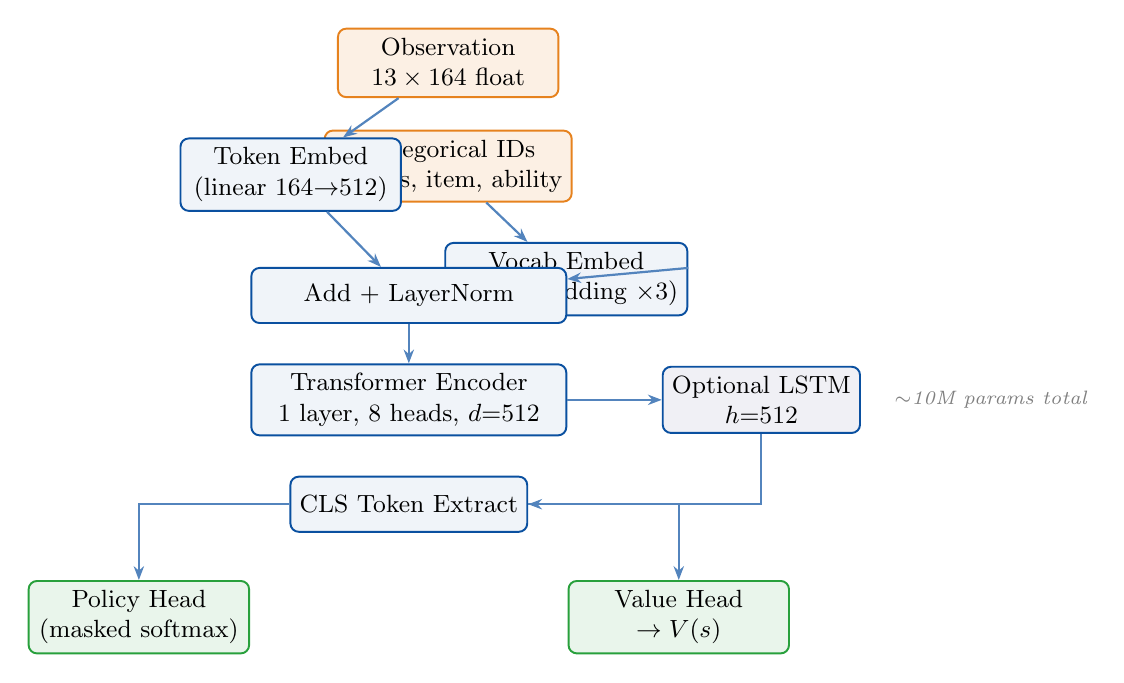
\begin{tikzpicture}[
    node distance=0.5cm and 0.8cm,
    block/.style={
      rectangle, draw=primaryBlue, fill=primaryBlue!6,
      rounded corners=3pt, minimum height=0.7cm, minimum width=2.8cm,
      font=\small, align=center, line width=0.7pt
    },
    io/.style={block, fill=accentOrange!12, draw=accentOrange},
    head/.style={block, fill=successGreen!10, draw=successGreen},
    arrow/.style={-{Stealth[length=5pt]}, thick, primaryBlue!70},
  ]
    % Input
    \node[io] (obs) {Observation\\$13 \times 164$ float};
    \node[io, below=0.4cm of obs] (ids) {Categorical IDs\\species, item, ability};

    % Embeddings
    \node[block, below=0.5cm of obs, xshift=-2cm] (tokemb) {Token Embed\\(linear 164$\to$512)};
    \node[block, below=0.5cm of ids, xshift=1.5cm] (vocabemb) {Vocab Embed\\(nn.Embedding $\times$3)};

    % Concat
    \node[block, below=0.7cm of tokemb, xshift=1.5cm, minimum width=4cm]
      (cat) {Add + LayerNorm};

    % Transformer
    \node[block, below=of cat, minimum width=4cm]
      (tf) {Transformer Encoder\\1 layer, 8 heads, $d{=}512$};

    % Optional LSTM
    \node[block, right=1.2cm of tf, minimum width=2.2cm, fill=lightGray]
      (lstm) {Optional LSTM\\$h{=}512$};

    % CLS token extraction
    \node[block, below=of tf] (cls) {CLS Token Extract};

    % Heads
    \node[head, below left=0.6cm and 0.5cm of cls] (policy) {Policy Head\\(masked softmax)};
    \node[head, below right=0.6cm and 0.5cm of cls] (value) {Value Head\\$\to V(s)$};

    % Arrows
    \draw[arrow] (obs) -- (tokemb);
    \draw[arrow] (ids) -- (vocabemb);
    \draw[arrow] (tokemb) -- (cat);
    \draw[arrow] (vocabemb) -- (cat);
    \draw[arrow] (cat) -- (tf);
    \draw[arrow] (tf) -- (lstm);
    \draw[arrow] (lstm) |- (cls);
    \draw[arrow] (cls) -| (policy);
    \draw[arrow] (cls) -| (value);

    % Param count
    \node[font=\scriptsize\itshape, text=gray, right=0.3cm of lstm]
      {${\sim}$10M params total};
  \end{tikzpicture}
\end{frame}

% --- Slide: Reward Design ---------------------------------------------------
\begin{frame}{Reward Design}
  \begin{columns}[T]
    \begin{column}{0.48\textwidth}
      \textbf{Reward components (per step):}
      \begin{center}
        \small
        \begin{tabularx}{\textwidth}{l X}
          \toprule
          \textbf{Signal} & \textbf{Weight / Value} \\
          \midrule
          Win bonus         & $+10$ \\
          Loss penalty      & $-10$ \\
          HP delta          & $\times 2.0$ \\
          Matchup quality   & $0.2$ \\
          Action quality    & $0.3$ \\
          \midrule
          \textbf{Reward scale} & $\mathbf{\times 0.1}$ \\
          \bottomrule
        \end{tabularx}
      \end{center}

      \vspace{0.3em}
      \small
      Returns scaled from $[-15, +15]$ to $[-1.5, +1.5]$.\\
      Discount: $\gamma = 0.97$, GAE $\lambda = 0.88$.
    \end{column}

    \begin{column}{0.48\textwidth}
      \begin{exampleblock}{Why reward scale = 0.1?}
        Without scaling, returns in $[-15, +15]$ made the value function
        unable to learn (explained variance $\sim 0.1$).
        Scaling to $[-1.5, +1.5]$ unlocked value learning: EV jumped to
        \textbf{0.72}. The single most impactful change in the project.
      \end{exampleblock}

      \vspace{0.3em}
      \textbf{Curriculum stages:}
      \begin{enumerate}\small
        \item Random warmup (70\% WR threshold)
        \item Self-play (85\% WR, 80/20 mix)
        \item Mixed terminal (50/30/20 heuristic/self/random)
      \end{enumerate}
    \end{column}
  \end{columns}
\end{frame}

% =============================================================================
% SECTION 4: DEVELOPMENT JOURNEY
% =============================================================================
\section{Development Journey}

% --- Slide: Debugging Timeline ----------------------------------------------
\begin{frame}{Development Timeline}
  \begin{center}
    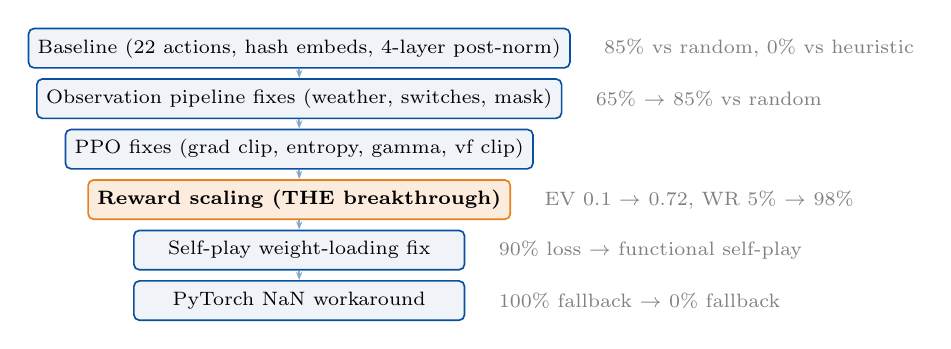
\begin{tikzpicture}[
      node distance=0.12cm,
      phase/.style={
        rectangle, draw=primaryBlue, fill=primaryBlue!6,
        rounded corners=2pt, minimum height=0.5cm, minimum width=4.2cm,
        font=\scriptsize, align=center, line width=0.6pt
      },
      breakthrough/.style={phase, fill=accentOrange!15, draw=accentOrange,
        font=\scriptsize\bfseries},
      arrow/.style={-{Stealth[length=3pt]}, primaryBlue!50, thick},
    ]
      \node[phase]        (p1) {Baseline (22 actions, hash embeds, 4-layer post-norm)};
      \node[phase, below=of p1]        (p2) {Observation pipeline fixes (weather, switches, mask)};
      \node[phase, below=of p2]        (p3) {PPO fixes (grad clip, entropy, gamma, vf clip)};
      \node[breakthrough, below=of p3] (p4) {Reward scaling (THE breakthrough)};
      \node[phase, below=of p4]        (p5) {Self-play weight-loading fix};
      \node[phase, below=of p5]        (p6) {PyTorch NaN workaround};

      \foreach \i/\j in {p1/p2, p2/p3, p3/p4, p4/p5, p5/p6} {
        \draw[arrow] (\i) -- (\j);
      }

      % Win rate annotations
      \node[font=\scriptsize, text=gray, right=0.3cm of p1] {85\% vs random, 0\% vs heuristic};
      \node[font=\scriptsize, text=gray, right=0.3cm of p2] {65\% $\to$ 85\% vs random};
      \node[font=\scriptsize, text=gray, right=0.3cm of p4] {EV 0.1 $\to$ 0.72, WR 5\% $\to$ 98\%};
      \node[font=\scriptsize, text=gray, right=0.3cm of p5] {90\% loss $\to$ functional self-play};
      \node[font=\scriptsize, text=gray, right=0.3cm of p6] {100\% fallback $\to$ 0\% fallback};
    \end{tikzpicture}
  \end{center}

  \vspace{0.3em}
  \textbf{Key takeaway:} Most ``progress'' came from fixing bugs and pipeline
  issues, not from architectural innovation. Systematic debugging was the
  primary driver.
\end{frame}

% --- Slide: Bug 1 - Gradient Starvation ------------------------------------
\begin{frame}{Critical Bug \#1: Gradient Starvation}
  \begin{columns}[T]
    \begin{column}{0.55\textwidth}
      \textbf{The problem:}
      \begin{itemize}\setlength{\itemsep}{0.3em}
        \item \texttt{grad\_clip} was set to \textbf{0.5}
        \item Total gradient norm: $\sim$65
        \item After clipping: all gradients scaled to \textbf{0.77\%} of original
        \item Transformer and embedding layers received near-zero updates
        \item Loss metrics looked \emph{normal} -- the failure was invisible
      \end{itemize}

      \vspace{0.5em}
      \textbf{The fix:} \texttt{grad\_clip}$\,= 0.5 \to 5.0$

      \vspace{0.3em}
      \textbf{Lesson:} Monitor gradient norms, not just losses.
    \end{column}

    \begin{column}{0.42\textwidth}
      \centering
      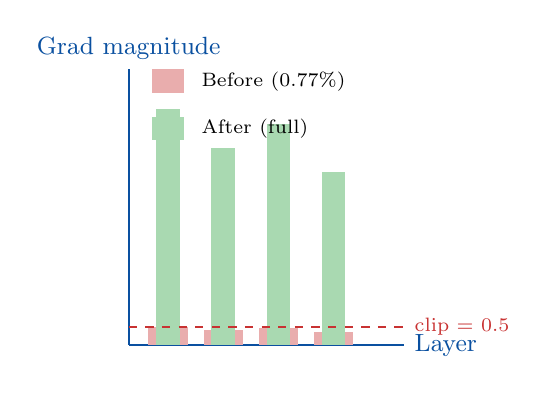
\begin{tikzpicture}
        \draw[thick, primaryBlue] (0,0) -- (0,3.5) node[above, font=\small] {Grad magnitude};
        \draw[thick, primaryBlue] (0,0) -- (3.5,0) node[right, font=\small] {Layer};

        % Before (clipped to 0.77%)
        \foreach \x/\h in {0.5/3.0, 1.2/2.5, 1.9/2.8, 2.6/2.2} {
          \fill[warnRed!40] (\x-0.25, 0) rectangle (\x+0.25, \h*0.077);
        }
        % After
        \foreach \x/\h in {0.5/3.0, 1.2/2.5, 1.9/2.8, 2.6/2.2} {
          \fill[successGreen!40] (\x-0.15, 0) rectangle (\x+0.15, \h);
        }

        % Clip line
        \draw[dashed, warnRed, thick] (0, 0.23) -- (3.5, 0.23)
          node[right, font=\scriptsize, text=warnRed] {clip = 0.5};

        % Legend
        \fill[warnRed!40] (0.3, 3.5) rectangle (0.7, 3.2);
        \node[right, font=\scriptsize] at (0.8, 3.35) {Before (0.77\%)};
        \fill[successGreen!40] (0.3, 2.9) rectangle (0.7, 2.6);
        \node[right, font=\scriptsize] at (0.8, 2.75) {After (full)};
      \end{tikzpicture}
    \end{column}
  \end{columns}
\end{frame}

% --- Slide: Bug 2 - Reward Scaling -----------------------------------------
\begin{frame}{Critical Bug \#2: Reward Scaling (The Breakthrough)}
  \begin{center}
    \small
    \begin{tabularx}{0.85\textwidth}{l c c}
      \toprule
      \textbf{Metric} & \textbf{Before Scaling} & \textbf{After Scaling} \\
      \midrule
      Returns range         & $[-15, +15]$          & $[-1.5, +1.5]$ \\
      Explained variance    & $\sim 0.1$ (sometimes neg.) & \textbf{0.53--0.87} (median 0.72) \\
      Value loss            & High, no trend        & \textbf{0.08--0.13} (converged by 15K steps) \\
      WR vs.\ heuristic     & $\sim 5\%$            & \textbf{98\%} (fixed teams) \\
      \bottomrule
    \end{tabularx}
  \end{center}

  \vspace{0.5em}
  \begin{exampleblock}{The Insight}
    For the entire project history, the value function was non-functional.
    A single change, \texttt{reward\_scale}$\,= 0.1$, caused explained
    variance to jump from $\sim 0.1$ to $0.72$ and unlocked competency
    against heuristic opponents.

    \vspace{0.3em}
    \textbf{Normalise the return scale before tuning anything else.}
    The value function must be able to learn before the policy can improve.
  \end{exampleblock}
\end{frame}

% --- Slide: Bug 3 - Self-Play & NaN ----------------------------------------
\begin{frame}{Critical Bug \#3: Self-Play Weight Loading + NaN}
  \begin{columns}[T]
    \begin{column}{0.48\textwidth}
      \textbf{Weight loading failure:}
      \begin{itemize}\setlength{\itemsep}{0.25em}
        \item \texttt{selfplay\_weights\_path} passed as \emph{relative} path
        \item Ray workers run from \texttt{/tmp/ray/\ldots/}
        \item Opponent played with \textbf{random init} weights
        \item \textbf{0 out of 12} workers loaded weights
        \item Hidden by silent \texttt{except: pass}
      \end{itemize}

      \vspace{0.4em}
      \textbf{Fix:} \texttt{os.path.abspath()} before passing to workers.
      Added diagnostic logging to detect load failures.

      \vspace{0.3em}
      \small\textit{Lesson: file paths in distributed systems must be absolute.}
    \end{column}

    \begin{column}{0.48\textwidth}
      \textbf{PyTorch 2.10 NaN bug:}
      \begin{itemize}\setlength{\itemsep}{0.25em}
        \item \texttt{TransformerEncoderLayer.forward()} with float
              \texttt{src\_mask} $\to$ NaN outputs
        \item Our learnable attention bias triggered it every forward pass
        \item NaN logits $\to$ \texttt{multinomial} error $\to$ fallback to
              random actions
        \item \textbf{100\% fallback rate}
      \end{itemize}

      \vspace{0.4em}
      \textbf{Fix:} Manual norm-first decomposition replacing the built-in
      \texttt{layer(x, src\_mask=bias)}.

      \vspace{0.3em}
      \small\textit{Lesson: framework bugs are real. Trusting internals without
      testing wastes weeks.}
    \end{column}
  \end{columns}
\end{frame}

% =============================================================================
% SECTION 5: RESULTS
% =============================================================================
\section{Results}

% --- Slide: M1 Results ------------------------------------------------------
\begin{frame}{Milestone 1: Fixed Teams}
  \begin{columns}[T]
    \begin{column}{0.45\textwidth}
      \begin{center}
        \begin{tabularx}{\textwidth}{l c}
          \toprule
          \textbf{Metric} & \textbf{Value} \\
          \midrule
          Skill score        & \textbf{0.9911} \\
          WR vs.\ random     & \textbf{100\%} \\
          WR vs.\ no-switch  & \textbf{96\%+} \\
          WR vs.\ heuristic  & \textbf{98\%} \\
          \bottomrule
        \end{tabularx}
      \end{center}

      \vspace{0.5em}
      \begin{exampleblock}{Conclusion}
        The architecture, observation pipeline, and reward design are
        \textbf{sufficient} when team information is available and teams
        are consistent.
      \end{exampleblock}
    \end{column}

    \begin{column}{0.52\textwidth}
      \textbf{Why does this work so well?}
      \begin{itemize}\setlength{\itemsep}{0.3em}
        \item \textbf{Known own team:} The agent learns one team's
              strategy deeply (memorises matchups, switching patterns).
        \item \textbf{Team preview:} All 6 opponent species visible from
              turn~1 $\to$ can plan switches proactively.
        \item \textbf{Low entropy:} Same team every battle eliminates
              the need for generalisation across team compositions.
      \end{itemize}

      \vspace{0.3em}
      \textbf{Hparam sweep confirms:}\\
      Most configurations reach 96--98\% vs.\ heuristic. Performance is
      \emph{architecture-agnostic} in this setting.
    \end{column}
  \end{columns}
\end{frame}

% --- Slide: M2 Results ------------------------------------------------------
\begin{frame}{Milestone 2: Random Teams \& The Entropy Problem}
  \begin{columns}[T]
    \begin{column}{0.48\textwidth}
      \begin{center}
        \small
        \begin{tabularx}{\textwidth}{l c}
          \toprule
          \textbf{Metric} & \textbf{Best Value} \\
          \midrule
          Skill score (best trial) & $\sim 0.37$ \\
          WR vs.\ heuristic        & $\sim 30\%$ \\
          \bottomrule
        \end{tabularx}
      \end{center}

      \vspace{0.4em}
      \textbf{Hparam sweep: 50 trials, 600K steps each}
      \begin{itemize}\setlength{\itemsep}{0.2em}
        \item Fixed teams: saturated at 96--98\% across most configs
        \item Random teams: \textbf{no configuration broke through}
        \item Problem is not opponent AI strength; it's team entropy
      \end{itemize}
    \end{column}

    \begin{column}{0.48\textwidth}
      \begin{alertblock}{The real insight}
        Our curriculum (opponent strength ramping: random $\to$ heuristic
        $\to$ self-play) turned out to be \textbf{less relevant} than
        initially thought.

        \vspace{0.3em}
        The dominant difficulty is \textbf{high entropy + partial
        observability} in random vs.\ random battles:
        \begin{itemize}\small
          \item No team preview (opponent revealed one-by-one)
          \item Every battle is a novel team matchup
          \item Qualitatively different: POMDP vs.\ near-MDP
        \end{itemize}
      \end{alertblock}
    \end{column}
  \end{columns}
\end{frame}

% --- Slide: Honest Assessment -----------------------------------------------
\begin{frame}{Honest Assessment}
  \begin{center}
    \small
    \begin{tabularx}{0.92\textwidth}{X X}
      \toprule
      \textbf{What works} & \textbf{What still needs work} \\
      \midrule
      Fixed teams: near-perfect (skill 0.99) &
        Random teams: skill 0.37, $\sim$30\% vs.\ heuristic \\
      Value function learns after reward scaling (EV 0.72) &
        Benchmark variance high at 50 eps/tier \\
      Self-play functional (0\% fallback) &
        LSTM end-to-end validation pending \\
      Distributed training stable at 48 envs &
        Gauntlet validation not automated \\
      MLflow produces complete, comparable metrics &
        Team builder (M3) not started \\
      Curriculum learning provides structured progression &
        Partial observability remains the core challenge \\
      \bottomrule
    \end{tabularx}
  \end{center}

  \vspace{0.5em}
  \textbf{Bottom line:} The engineering foundation is solid and M1 is solved.
  The remaining challenge is fundamental: generalisation under hidden
  information with high team entropy.
\end{frame}

% =============================================================================
% SECTION 6: LIVE DEMO
% =============================================================================
\section{Live Demo}

\begin{frame}[plain]
  \begin{center}
    \vfill
    {\Huge\color{primaryBlue} Live Demo}\\[1em]
    {\large Agent vs.\ Heuristic Opponent}\\[0.5em]
    {\small\color{gray} Fixed team, gen8customgamenogimmicks format}
    \vfill
  \end{center}
\end{frame}

% =============================================================================
% SECTION 7: CONCLUSIONS
% =============================================================================
\section{Conclusions \& Next Steps}

% --- Slide: Lessons Learned -------------------------------------------------
\begin{frame}{Lessons Learned}
  \begin{enumerate}\setlength{\itemsep}{0.5em}
    \item \textbf{Normalise the return scale first.}
          Reward scaling ($\times 0.1$) was more impactful than any
          architectural change. The value function must learn before the
          policy can improve.

    \item \textbf{Systematic debugging $>$ throwing compute at the problem.}
          Three observation bugs collectively affected 14\% of steps.
          A silent weight-loading bug wasted weeks of self-play training.

    \item \textbf{Reward design outweighs architecture tuning.}
          The biggest gains came from fixing observation bugs (WR 65\%
          $\to$ 85\%) and reward scaling (WR 5\% $\to$ 98\%), not from
          model changes.

    \item \textbf{Curriculum design must target the right axis of difficulty.}
          Opponent strength was less important than information availability.
          High entropy in team composition is the real bottleneck.

    \item \textbf{Framework bugs happen.}
          PyTorch 2.10 NaN with float attention masks required manual
          decomposition. Trusting framework internals wastes time.
  \end{enumerate}
\end{frame}

% --- Slide: Future Work -----------------------------------------------------
\begin{frame}{Next Steps \& Future Work}
  \begin{columns}[T]
    \begin{column}{0.48\textwidth}
      \textbf{Short term (continuing the project):}
      \begin{itemize}\setlength{\itemsep}{0.2em}
        \item Gradually expand from fixed teams at win-rate thresholds
              (bridge M1 $\to$ M2)
        \item Complete-information random vs.\ random as controlled
              experiment
        \item Increase benchmark stability (100+ eps/tier)
        \item Validate LSTM benefit in A/B test
      \end{itemize}
    \end{column}

    \begin{column}{0.48\textwidth}
      \textbf{Longer term:}
      \begin{itemize}\setlength{\itemsep}{0.2em}
        \item \textbf{Pretraining on Showdown logs} $+$ RL finetuning:
              likely the highest-impact change not attempted
        \item Auxiliary tasks (move prediction, state-value supervision)
        \item Milestone~3: team composition model
        \item Milestone~4: full Nuzlocke gauntlet
      \end{itemize}
    \end{column}
  \end{columns}

  \vspace{0.6em}
  \begin{block}{Project Outlook}
    The project continues beyond the DSPRO2 module. The engineering
    foundation (distributed training, validation, experiment tracking) is
    solid. The remaining challenge: generalisation under partial
    observability.
  \end{block}
\end{frame}

% --- Slide: Q&A -------------------------------------------------------------
\begin{frame}[plain]
  \begin{center}
    \vfill
    {\Huge\color{primaryBlue} Questions?}\\[1.5em]
    {\large Thank you for your attention}\\[1em]
    {\small Tristan Muri, Marvin Hueber, Viacheslav Godovskii, Alex Liubov}\\[0.5em]
    {\small\color{gray} DSPRO2 FS26 -- Hochschule Luzern}
    \vfill
  \end{center}
\end{frame}

\end{document}
